\documentclass[crop,tikz]{standalone}
\usepackage{graphicx}
\usepackage{tabularx}
\begin{document}
\begin{tikzpicture}
  \node[inner sep=0pt, anchor=north west] at (1.7,-0.2)
{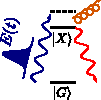
\includegraphics[width=2.3cm]{sketch_phonon7.pdf}};

  \node[inner sep=0pt, anchor=north west]  at (0,0)
    {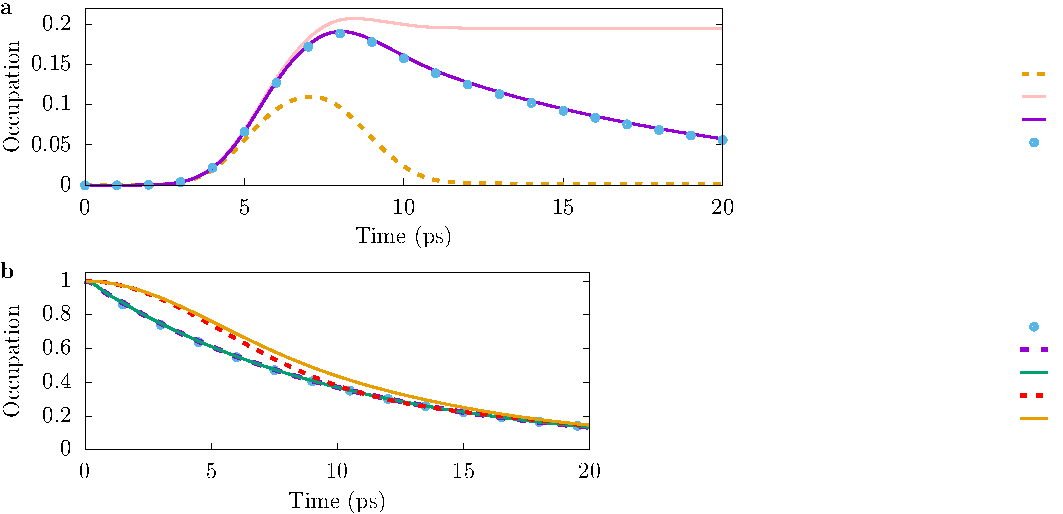
\includegraphics{fig3_data.pdf}};

\node[inner sep=0pt, anchor=south east, scale=0.9] at (17,-2.6) {  %16.2
\begin{tabular}{ll}
\textbf{Phonons:} & \textbf{Photons:} \\[0.5mm]
none & Lindblad \\
ACE & none \\
ACE & ACE \\
iQUAPI & Lindblad
\end{tabular}
};

\node[inner sep=0pt, anchor=south east, scale=0.9] at (17,-7.29) {
\begin{tabular}{cll}
\textbf{Bandwidth:} &\textbf{Phonons:} & \textbf{Photons:} \\[0.5mm]
&iQUAPI & Lindblad \\
$\hbar\times 10$ ps$^{-1}$ & none & ACE \\
$\hbar\times 10$ ps$^{-1}$ & ACE & ACE \\
$\hbar\times 0.4$ ps$^{-1}$ & none & ACE \\
$\hbar\times 0.4$ ps$^{-1}$ & ACE & ACE 
\end{tabular}
};

%\draw[step=1.0,black,thin] (0.,0.) grid (14,-14);
\end{tikzpicture}
\end{document}
